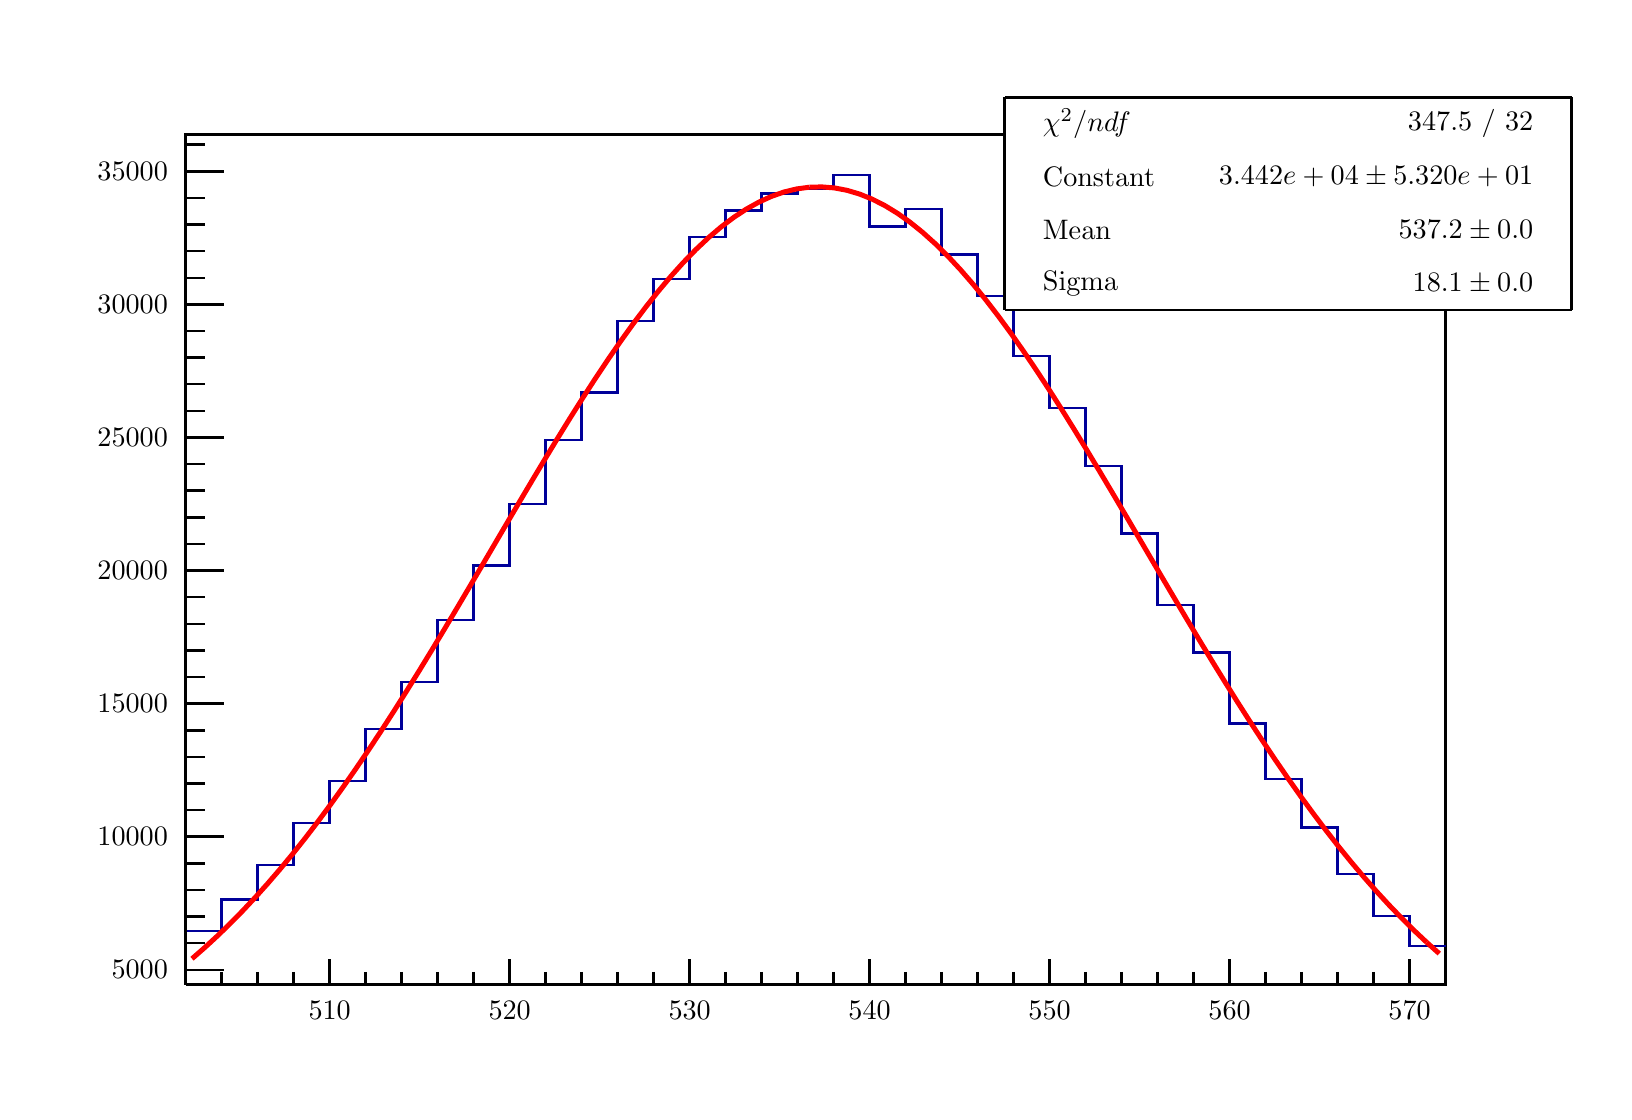
\begin{tikzpicture}
\pgfdeclareplotmark{cross} {
\pgfpathmoveto{\pgfpoint{-0.3\pgfplotmarksize}{\pgfplotmarksize}}
\pgfpathlineto{\pgfpoint{+0.3\pgfplotmarksize}{\pgfplotmarksize}}
\pgfpathlineto{\pgfpoint{+0.3\pgfplotmarksize}{0.3\pgfplotmarksize}}
\pgfpathlineto{\pgfpoint{+1\pgfplotmarksize}{0.3\pgfplotmarksize}}
\pgfpathlineto{\pgfpoint{+1\pgfplotmarksize}{-0.3\pgfplotmarksize}}
\pgfpathlineto{\pgfpoint{+0.3\pgfplotmarksize}{-0.3\pgfplotmarksize}}
\pgfpathlineto{\pgfpoint{+0.3\pgfplotmarksize}{-1.\pgfplotmarksize}}
\pgfpathlineto{\pgfpoint{-0.3\pgfplotmarksize}{-1.\pgfplotmarksize}}
\pgfpathlineto{\pgfpoint{-0.3\pgfplotmarksize}{-0.3\pgfplotmarksize}}
\pgfpathlineto{\pgfpoint{-1.\pgfplotmarksize}{-0.3\pgfplotmarksize}}
\pgfpathlineto{\pgfpoint{-1.\pgfplotmarksize}{0.3\pgfplotmarksize}}
\pgfpathlineto{\pgfpoint{-0.3\pgfplotmarksize}{0.3\pgfplotmarksize}}
\pgfpathclose
\pgfusepathqstroke
}
\pgfdeclareplotmark{cross*} {
\pgfpathmoveto{\pgfpoint{-0.3\pgfplotmarksize}{\pgfplotmarksize}}
\pgfpathlineto{\pgfpoint{+0.3\pgfplotmarksize}{\pgfplotmarksize}}
\pgfpathlineto{\pgfpoint{+0.3\pgfplotmarksize}{0.3\pgfplotmarksize}}
\pgfpathlineto{\pgfpoint{+1\pgfplotmarksize}{0.3\pgfplotmarksize}}
\pgfpathlineto{\pgfpoint{+1\pgfplotmarksize}{-0.3\pgfplotmarksize}}
\pgfpathlineto{\pgfpoint{+0.3\pgfplotmarksize}{-0.3\pgfplotmarksize}}
\pgfpathlineto{\pgfpoint{+0.3\pgfplotmarksize}{-1.\pgfplotmarksize}}
\pgfpathlineto{\pgfpoint{-0.3\pgfplotmarksize}{-1.\pgfplotmarksize}}
\pgfpathlineto{\pgfpoint{-0.3\pgfplotmarksize}{-0.3\pgfplotmarksize}}
\pgfpathlineto{\pgfpoint{-1.\pgfplotmarksize}{-0.3\pgfplotmarksize}}
\pgfpathlineto{\pgfpoint{-1.\pgfplotmarksize}{0.3\pgfplotmarksize}}
\pgfpathlineto{\pgfpoint{-0.3\pgfplotmarksize}{0.3\pgfplotmarksize}}
\pgfpathclose
\pgfusepathqfillstroke
}
\pgfdeclareplotmark{newstar} {
\pgfpathmoveto{\pgfqpoint{0pt}{\pgfplotmarksize}}
\pgfpathlineto{\pgfqpointpolar{44}{0.5\pgfplotmarksize}}
\pgfpathlineto{\pgfqpointpolar{18}{\pgfplotmarksize}}
\pgfpathlineto{\pgfqpointpolar{-20}{0.5\pgfplotmarksize}}
\pgfpathlineto{\pgfqpointpolar{-54}{\pgfplotmarksize}}
\pgfpathlineto{\pgfqpointpolar{-90}{0.5\pgfplotmarksize}}
\pgfpathlineto{\pgfqpointpolar{234}{\pgfplotmarksize}}
\pgfpathlineto{\pgfqpointpolar{198}{0.5\pgfplotmarksize}}
\pgfpathlineto{\pgfqpointpolar{162}{\pgfplotmarksize}}
\pgfpathlineto{\pgfqpointpolar{134}{0.5\pgfplotmarksize}}
\pgfpathclose
\pgfusepathqstroke
}
\pgfdeclareplotmark{newstar*} {
\pgfpathmoveto{\pgfqpoint{0pt}{\pgfplotmarksize}}
\pgfpathlineto{\pgfqpointpolar{44}{0.5\pgfplotmarksize}}
\pgfpathlineto{\pgfqpointpolar{18}{\pgfplotmarksize}}
\pgfpathlineto{\pgfqpointpolar{-20}{0.5\pgfplotmarksize}}
\pgfpathlineto{\pgfqpointpolar{-54}{\pgfplotmarksize}}
\pgfpathlineto{\pgfqpointpolar{-90}{0.5\pgfplotmarksize}}
\pgfpathlineto{\pgfqpointpolar{234}{\pgfplotmarksize}}
\pgfpathlineto{\pgfqpointpolar{198}{0.5\pgfplotmarksize}}
\pgfpathlineto{\pgfqpointpolar{162}{\pgfplotmarksize}}
\pgfpathlineto{\pgfqpointpolar{134}{0.5\pgfplotmarksize}}
\pgfpathclose
\pgfusepathqfillstroke
}
\definecolor{c}{rgb}{1,1,1};
\draw [color=c, fill=c] (0,0) rectangle (20,13.4957);
\draw [color=c, fill=c] (2,1.34957) rectangle (18,12.1461);
\definecolor{c}{rgb}{0,0,0};
\draw [c,line width=0.9] (2,1.34957) -- (2,12.1461) -- (18,12.1461) -- (18,1.34957) -- (2,1.34957);
\definecolor{c}{rgb}{1,1,1};
\draw [color=c, fill=c] (2,1.34957) rectangle (18,12.1461);
\definecolor{c}{rgb}{0,0,0};
\draw [c,line width=0.9] (2,1.34957) -- (2,12.1461) -- (18,12.1461) -- (18,1.34957) -- (2,1.34957);
\definecolor{c}{rgb}{0,0,0.6};
\draw [c,line width=0.9] (2,2.03357) -- (2.45714,2.03357) -- (2.45714,2.42939) -- (2.91429,2.42939) -- (2.91429,2.86815) -- (3.37143,2.86815) -- (3.37143,3.40188) -- (3.82857,3.40188) -- (3.82857,3.93528) -- (4.28571,3.93528) -- (4.28571,4.59442) --
 (4.74286,4.59442) -- (4.74286,5.19508) -- (5.2,5.19508) -- (5.2,5.98132) -- (5.65714,5.98132) -- (5.65714,6.67392) -- (6.11429,6.67392) -- (6.11429,7.45407) -- (6.57143,7.45407) -- (6.57143,8.26566) -- (7.02857,8.26566) -- (7.02857,8.8697) --
 (7.48571,8.8697) -- (7.48571,9.77661) -- (7.94286,9.77661) -- (7.94286,10.308) -- (8.4,10.308) -- (8.4,10.8417) -- (8.85714,10.8417) -- (8.85714,11.1777) -- (9.31429,11.1777) -- (9.31429,11.3961) -- (9.77143,11.3961) -- (9.77143,11.4606) --
 (10.2286,11.4606) -- (10.2286,11.632) -- (10.6857,11.632) -- (10.6857,10.9806) -- (11.1429,10.9806) -- (11.1429,11.2017) -- (11.6,11.2017) -- (11.6,10.6196) -- (12.0571,10.6196) -- (12.0571,10.0933) -- (12.5143,10.0933) -- (12.5143,9.33347) --
 (12.9714,9.33347) -- (12.9714,8.675) -- (13.4286,8.675) -- (13.4286,7.93271) -- (13.8857,7.93271) -- (13.8857,7.07887) -- (14.3429,7.07887) -- (14.3429,6.17162) -- (14.8,6.17162) -- (14.8,5.56555) -- (15.2571,5.56555) -- (15.2571,4.66405) --
 (15.7143,4.66405) -- (15.7143,3.9613) -- (16.1714,3.9613) -- (16.1714,3.34475) -- (16.6286,3.34475) -- (16.6286,2.75153) -- (17.0857,2.75153) -- (17.0857,2.2205) -- (17.5429,2.2205) -- (17.5429,1.83921) -- (18,1.83921);
\definecolor{c}{rgb}{1,0,0};
\draw [c,line width=1.8] (2.08,1.67835) -- (2.24,1.8182) -- (2.4,1.96557) -- (2.56,2.12055) -- (2.72,2.28323) -- (2.88,2.45366) -- (3.04,2.63184) -- (3.2,2.81776) -- (3.36,3.01137) -- (3.52,3.21255) -- (3.68,3.42119) -- (3.84,3.63709) -- (4,3.86003)
 -- (4.16,4.08974) -- (4.32,4.32591) -- (4.48,4.56815) -- (4.64,4.81607) -- (4.8,5.06919) -- (4.96,5.32701) -- (5.12,5.58897) -- (5.28,5.85446) -- (5.44,6.12285) -- (5.6,6.39343) -- (5.76,6.66547) -- (5.92,6.93822) -- (6.08,7.21086) -- (6.24,7.48255)
 -- (6.4,7.75245) -- (6.56,8.01966) -- (6.72,8.28328) -- (6.88,8.54239) -- (7.04,8.79608) -- (7.2,9.04341) -- (7.36,9.28345) -- (7.52,9.5153) -- (7.68,9.73805) -- (7.84,9.95081) -- (8,10.1527) -- (8.16,10.343) -- (8.32,10.5208) -- (8.48,10.6854) --
 (8.64,10.8361) -- (8.8,10.9722) -- (8.96,11.0932) -- (9.12,11.1985) -- (9.28,11.2877) -- (9.44,11.3604) -- (9.6,11.4162) -- (9.76,11.455) -- (9.92,11.4764);
\draw [c,line width=1.8] (9.92,11.4764) -- (10.08,11.4805) -- (10.24,11.4672) -- (10.4,11.4366) -- (10.56,11.3888) -- (10.72,11.3241) -- (10.88,11.2426) -- (11.04,11.1448) -- (11.2,11.0311) -- (11.36,10.9021) -- (11.52,10.7582) -- (11.68,10.6) --
 (11.84,10.4284) -- (12,10.2439) -- (12.16,10.0474) -- (12.32,9.83961) -- (12.48,9.62146) -- (12.64,9.3938) -- (12.8,9.1575) -- (12.96,8.91349) -- (13.12,8.66268) -- (13.28,8.40601) -- (13.44,8.1444) -- (13.6,7.87877) -- (13.76,7.61003) --
 (13.92,7.33907) -- (14.08,7.06677) -- (14.24,6.79397) -- (14.4,6.5215) -- (14.56,6.25014) -- (14.72,5.98063) -- (14.88,5.71369) -- (15.04,5.44998) -- (15.2,5.19014) -- (15.36,4.93474) -- (15.52,4.68431) -- (15.68,4.43934) -- (15.84,4.20026) --
 (16,3.96747) -- (16.16,3.7413) -- (16.32,3.52205) -- (16.48,3.30996) -- (16.64,3.10524) -- (16.8,2.90805) -- (16.96,2.7185) -- (17.12,2.53666) -- (17.28,2.36258) -- (17.44,2.19626) -- (17.6,2.03765) -- (17.76,1.88671);
\draw [c,line width=1.8] (17.76,1.88671) -- (17.92,1.74333);
\definecolor{c}{rgb}{1,1,1};
\draw [color=c, fill=c] (12.4,9.91934) rectangle (19.6,12.6185);
\definecolor{c}{rgb}{0,0,0};
\draw [c,line width=0.9] (12.4,9.91934) -- (19.6,9.91934);
\draw [c,line width=0.9] (19.6,9.91934) -- (19.6,12.6185);
\draw [c,line width=0.9] (19.6,12.6185) -- (12.4,12.6185);
\draw [c,line width=0.9] (12.4,12.6185) -- (12.4,9.91934);
\draw [anchor= west] (12.76,12.2811) node[scale=1.01821, color=c, rotate=0]{$\chi^{2} / ndf $};
\draw [anchor= east] (19.24,12.2811) node[scale=1.01821, color=c, rotate=0]{ 347.5 / 32};
\draw [anchor= west] (12.76,11.6063) node[scale=1.01821, color=c, rotate=0]{Constant };
\draw [anchor= east] (19.24,11.6063) node[scale=1.01821, color=c, rotate=0]{$ 3.442e+04 \pm 5.320e+01$};
\draw [anchor= west] (12.76,10.9315) node[scale=1.01821, color=c, rotate=0]{Mean     };
\draw [anchor= east] (19.24,10.9315) node[scale=1.01821, color=c, rotate=0]{$ 537.2 \pm 0.0$};
\draw [anchor= west] (12.76,10.2567) node[scale=1.01821, color=c, rotate=0]{Sigma    };
\draw [anchor= east] (19.24,10.2567) node[scale=1.01821, color=c, rotate=0]{$  18.1 \pm 0.0$};
\draw [c,line width=0.9] (2,1.34957) -- (18,1.34957);
\draw [c,line width=0.9] (3.82857,1.67347) -- (3.82857,1.34957);
\draw [c,line width=0.9] (4.28571,1.51152) -- (4.28571,1.34957);
\draw [c,line width=0.9] (4.74286,1.51152) -- (4.74286,1.34957);
\draw [c,line width=0.9] (5.2,1.51152) -- (5.2,1.34957);
\draw [c,line width=0.9] (5.65714,1.51152) -- (5.65714,1.34957);
\draw [c,line width=0.9] (6.11429,1.67347) -- (6.11429,1.34957);
\draw [c,line width=0.9] (6.57143,1.51152) -- (6.57143,1.34957);
\draw [c,line width=0.9] (7.02857,1.51152) -- (7.02857,1.34957);
\draw [c,line width=0.9] (7.48571,1.51152) -- (7.48571,1.34957);
\draw [c,line width=0.9] (7.94286,1.51152) -- (7.94286,1.34957);
\draw [c,line width=0.9] (8.4,1.67347) -- (8.4,1.34957);
\draw [c,line width=0.9] (8.85714,1.51152) -- (8.85714,1.34957);
\draw [c,line width=0.9] (9.31429,1.51152) -- (9.31429,1.34957);
\draw [c,line width=0.9] (9.77143,1.51152) -- (9.77143,1.34957);
\draw [c,line width=0.9] (10.2286,1.51152) -- (10.2286,1.34957);
\draw [c,line width=0.9] (10.6857,1.67347) -- (10.6857,1.34957);
\draw [c,line width=0.9] (11.1429,1.51152) -- (11.1429,1.34957);
\draw [c,line width=0.9] (11.6,1.51152) -- (11.6,1.34957);
\draw [c,line width=0.9] (12.0571,1.51152) -- (12.0571,1.34957);
\draw [c,line width=0.9] (12.5143,1.51152) -- (12.5143,1.34957);
\draw [c,line width=0.9] (12.9714,1.67347) -- (12.9714,1.34957);
\draw [c,line width=0.9] (13.4286,1.51152) -- (13.4286,1.34957);
\draw [c,line width=0.9] (13.8857,1.51152) -- (13.8857,1.34957);
\draw [c,line width=0.9] (14.3429,1.51152) -- (14.3429,1.34957);
\draw [c,line width=0.9] (14.8,1.51152) -- (14.8,1.34957);
\draw [c,line width=0.9] (15.2571,1.67347) -- (15.2571,1.34957);
\draw [c,line width=0.9] (15.7143,1.51152) -- (15.7143,1.34957);
\draw [c,line width=0.9] (16.1714,1.51152) -- (16.1714,1.34957);
\draw [c,line width=0.9] (16.6286,1.51152) -- (16.6286,1.34957);
\draw [c,line width=0.9] (17.0857,1.51152) -- (17.0857,1.34957);
\draw [c,line width=0.9] (17.5429,1.67347) -- (17.5429,1.34957);
\draw [c,line width=0.9] (3.82857,1.67347) -- (3.82857,1.34957);
\draw [c,line width=0.9] (3.37143,1.51152) -- (3.37143,1.34957);
\draw [c,line width=0.9] (2.91429,1.51152) -- (2.91429,1.34957);
\draw [c,line width=0.9] (2.45714,1.51152) -- (2.45714,1.34957);
\draw [c,line width=0.9] (2,1.51152) -- (2,1.34957);
\draw [c,line width=0.9] (17.5429,1.67347) -- (17.5429,1.34957);
\draw [c,line width=0.9] (18,1.51152) -- (18,1.34957);
\draw [anchor=base] (3.82857,0.904212) node[scale=1.01821, color=c, rotate=0]{510};
\draw [anchor=base] (6.11429,0.904212) node[scale=1.01821, color=c, rotate=0]{520};
\draw [anchor=base] (8.4,0.904212) node[scale=1.01821, color=c, rotate=0]{530};
\draw [anchor=base] (10.6857,0.904212) node[scale=1.01821, color=c, rotate=0]{540};
\draw [anchor=base] (12.9714,0.904212) node[scale=1.01821, color=c, rotate=0]{550};
\draw [anchor=base] (15.2571,0.904212) node[scale=1.01821, color=c, rotate=0]{560};
\draw [anchor=base] (17.5429,0.904212) node[scale=1.01821, color=c, rotate=0]{570};
\draw [c,line width=0.9] (2,1.34957) -- (2,12.1461);
\draw [c,line width=0.9] (2.48,1.5377) -- (2,1.5377);
\draw [c,line width=0.9] (2.24,1.87572) -- (2,1.87572);
\draw [c,line width=0.9] (2.24,2.21374) -- (2,2.21374);
\draw [c,line width=0.9] (2.24,2.55176) -- (2,2.55176);
\draw [c,line width=0.9] (2.24,2.88978) -- (2,2.88978);
\draw [c,line width=0.9] (2.48,3.2278) -- (2,3.2278);
\draw [c,line width=0.9] (2.24,3.56582) -- (2,3.56582);
\draw [c,line width=0.9] (2.24,3.90384) -- (2,3.90384);
\draw [c,line width=0.9] (2.24,4.24186) -- (2,4.24186);
\draw [c,line width=0.9] (2.24,4.57988) -- (2,4.57988);
\draw [c,line width=0.9] (2.48,4.9179) -- (2,4.9179);
\draw [c,line width=0.9] (2.24,5.25592) -- (2,5.25592);
\draw [c,line width=0.9] (2.24,5.59395) -- (2,5.59395);
\draw [c,line width=0.9] (2.24,5.93197) -- (2,5.93197);
\draw [c,line width=0.9] (2.24,6.26999) -- (2,6.26999);
\draw [c,line width=0.9] (2.48,6.60801) -- (2,6.60801);
\draw [c,line width=0.9] (2.24,6.94603) -- (2,6.94603);
\draw [c,line width=0.9] (2.24,7.28405) -- (2,7.28405);
\draw [c,line width=0.9] (2.24,7.62207) -- (2,7.62207);
\draw [c,line width=0.9] (2.24,7.96009) -- (2,7.96009);
\draw [c,line width=0.9] (2.48,8.29811) -- (2,8.29811);
\draw [c,line width=0.9] (2.24,8.63613) -- (2,8.63613);
\draw [c,line width=0.9] (2.24,8.97415) -- (2,8.97415);
\draw [c,line width=0.9] (2.24,9.31217) -- (2,9.31217);
\draw [c,line width=0.9] (2.24,9.65019) -- (2,9.65019);
\draw [c,line width=0.9] (2.48,9.98821) -- (2,9.98821);
\draw [c,line width=0.9] (2.24,10.3262) -- (2,10.3262);
\draw [c,line width=0.9] (2.24,10.6643) -- (2,10.6643);
\draw [c,line width=0.9] (2.24,11.0023) -- (2,11.0023);
\draw [c,line width=0.9] (2.24,11.3403) -- (2,11.3403);
\draw [c,line width=0.9] (2.48,11.6783) -- (2,11.6783);
\draw [c,line width=0.9] (2.48,1.5377) -- (2,1.5377);
\draw [c,line width=0.9] (2.48,11.6783) -- (2,11.6783);
\draw [c,line width=0.9] (2.24,12.0163) -- (2,12.0163);
\draw [anchor= east] (1.9,1.5377) node[scale=1.01821, color=c, rotate=0]{5000};
\draw [anchor= east] (1.9,3.2278) node[scale=1.01821, color=c, rotate=0]{10000};
\draw [anchor= east] (1.9,4.9179) node[scale=1.01821, color=c, rotate=0]{15000};
\draw [anchor= east] (1.9,6.60801) node[scale=1.01821, color=c, rotate=0]{20000};
\draw [anchor= east] (1.9,8.29811) node[scale=1.01821, color=c, rotate=0]{25000};
\draw [anchor= east] (1.9,9.98821) node[scale=1.01821, color=c, rotate=0]{30000};
\draw [anchor= east] (1.9,11.6783) node[scale=1.01821, color=c, rotate=0]{35000};
\definecolor{c}{rgb}{1,1,1};
\draw [color=c, fill=c] (12.4,9.91934) rectangle (19.6,12.6185);
\definecolor{c}{rgb}{0,0,0};
\draw [c,line width=0.9] (12.4,9.91934) -- (19.6,9.91934);
\draw [c,line width=0.9] (19.6,9.91934) -- (19.6,12.6185);
\draw [c,line width=0.9] (19.6,12.6185) -- (12.4,12.6185);
\draw [c,line width=0.9] (12.4,12.6185) -- (12.4,9.91934);
\draw [anchor= west] (12.76,12.2811) node[scale=1.01821, color=c, rotate=0]{$\chi^{2} / ndf $};
\draw [anchor= east] (19.24,12.2811) node[scale=1.01821, color=c, rotate=0]{ 347.5 / 32};
\draw [anchor= west] (12.76,11.6063) node[scale=1.01821, color=c, rotate=0]{Constant };
\draw [anchor= east] (19.24,11.6063) node[scale=1.01821, color=c, rotate=0]{$ 3.442e+04 \pm 5.320e+01$};
\draw [anchor= west] (12.76,10.9315) node[scale=1.01821, color=c, rotate=0]{Mean     };
\draw [anchor= east] (19.24,10.9315) node[scale=1.01821, color=c, rotate=0]{$ 537.2 \pm 0.0$};
\draw [anchor= west] (12.76,10.2567) node[scale=1.01821, color=c, rotate=0]{Sigma    };
\draw [anchor= east] (19.24,10.2567) node[scale=1.01821, color=c, rotate=0]{$  18.1 \pm 0.0$};
\end{tikzpicture}
